\documentclass[twoside]{book}

% Packages required by doxygen
\usepackage{fixltx2e}
\usepackage{calc}
\usepackage{doxygen}
\usepackage[export]{adjustbox} % also loads graphicx
\usepackage{graphicx}
\usepackage[utf8]{inputenc}
\usepackage{makeidx}
\usepackage{multicol}
\usepackage{multirow}
\PassOptionsToPackage{warn}{textcomp}
\usepackage{textcomp}
\usepackage[nointegrals]{wasysym}
\usepackage[table]{xcolor}

% Font selection
\usepackage[T1]{fontenc}
\usepackage[scaled=.90]{helvet}
\usepackage{courier}
\usepackage{amssymb}
\usepackage{sectsty}
\renewcommand{\familydefault}{\sfdefault}
\allsectionsfont{%
  \fontseries{bc}\selectfont%
  \color{darkgray}%
}
\renewcommand{\DoxyLabelFont}{%
  \fontseries{bc}\selectfont%
  \color{darkgray}%
}
\newcommand{\+}{\discretionary{\mbox{\scriptsize$\hookleftarrow$}}{}{}}

% Page & text layout
\usepackage{geometry}
\geometry{%
  a4paper,%
  top=2.5cm,%
  bottom=2.5cm,%
  left=2.5cm,%
  right=2.5cm%
}
\tolerance=750
\hfuzz=15pt
\hbadness=750
\setlength{\emergencystretch}{15pt}
\setlength{\parindent}{0cm}
\setlength{\parskip}{3ex plus 2ex minus 2ex}
\makeatletter
\renewcommand{\paragraph}{%
  \@startsection{paragraph}{4}{0ex}{-1.0ex}{1.0ex}{%
    \normalfont\normalsize\bfseries\SS@parafont%
  }%
}
\renewcommand{\subparagraph}{%
  \@startsection{subparagraph}{5}{0ex}{-1.0ex}{1.0ex}{%
    \normalfont\normalsize\bfseries\SS@subparafont%
  }%
}
\makeatother

% Headers & footers
\usepackage{fancyhdr}
\pagestyle{fancyplain}
\fancyhead[LE]{\fancyplain{}{\bfseries\thepage}}
\fancyhead[CE]{\fancyplain{}{}}
\fancyhead[RE]{\fancyplain{}{\bfseries\leftmark}}
\fancyhead[LO]{\fancyplain{}{\bfseries\rightmark}}
\fancyhead[CO]{\fancyplain{}{}}
\fancyhead[RO]{\fancyplain{}{\bfseries\thepage}}
\fancyfoot[LE]{\fancyplain{}{}}
\fancyfoot[CE]{\fancyplain{}{}}
\fancyfoot[RE]{\fancyplain{}{\bfseries\scriptsize Generated by Doxygen }}
\fancyfoot[LO]{\fancyplain{}{\bfseries\scriptsize Generated by Doxygen }}
\fancyfoot[CO]{\fancyplain{}{}}
\fancyfoot[RO]{\fancyplain{}{}}
\renewcommand{\footrulewidth}{0.4pt}
\renewcommand{\chaptermark}[1]{%
  \markboth{#1}{}%
}
\renewcommand{\sectionmark}[1]{%
  \markright{\thesection\ #1}%
}

% Indices & bibliography
\usepackage{natbib}
\usepackage[titles]{tocloft}
\setcounter{tocdepth}{3}
\setcounter{secnumdepth}{5}
\makeindex

% Hyperlinks (required, but should be loaded last)
\usepackage{ifpdf}
\ifpdf
  \usepackage[pdftex,pagebackref=true]{hyperref}
\else
  \usepackage[ps2pdf,pagebackref=true]{hyperref}
\fi
\hypersetup{%
  colorlinks=true,%
  linkcolor=blue,%
  citecolor=blue,%
  unicode%
}

% Custom commands
\newcommand{\clearemptydoublepage}{%
  \newpage{\pagestyle{empty}\cleardoublepage}%
}

\usepackage{caption}
\captionsetup{labelsep=space,justification=centering,font={bf},singlelinecheck=off,skip=4pt,position=top}

%===== C O N T E N T S =====

\begin{document}

% Titlepage & ToC
\hypersetup{pageanchor=false,
             bookmarksnumbered=true,
             pdfencoding=unicode
            }
\pagenumbering{alph}
\begin{titlepage}
\vspace*{7cm}
\begin{center}%
{\Large Robot Controller }\\
\vspace*{1cm}
{\large Generated by Doxygen 1.8.13}\\
\end{center}
\end{titlepage}
\clearemptydoublepage
\pagenumbering{roman}
\tableofcontents
\clearemptydoublepage
\pagenumbering{arabic}
\hypersetup{pageanchor=true}

%--- Begin generated contents ---
\chapter{Class Index}
\section{Class List}
Here are the classes, structs, unions and interfaces with brief descriptions\+:\begin{DoxyCompactList}
\item\contentsline{section}{\hyperlink{classAckermann}{Ackermann} \\*Implementation of an \hyperlink{classAckermann}{Ackermann} Controller }{\pageref{classAckermann}}{}
\item\contentsline{section}{\hyperlink{classgnuplotio_1_1ArrayTraits}{gnuplotio\+::\+Array\+Traits$<$ T, Enable $>$} }{\pageref{classgnuplotio_1_1ArrayTraits}}{}
\item\contentsline{section}{\hyperlink{classgnuplotio_1_1ArrayTraits_3_01std_1_1pair_3_01T_00_01U_01_4_01_4}{gnuplotio\+::\+Array\+Traits$<$ std\+::pair$<$ T, U $>$ $>$} }{\pageref{classgnuplotio_1_1ArrayTraits_3_01std_1_1pair_3_01T_00_01U_01_4_01_4}}{}
\item\contentsline{section}{\hyperlink{classgnuplotio_1_1ArrayTraits_3_01T_01_6_01_4}{gnuplotio\+::\+Array\+Traits$<$ T \& $>$} }{\pageref{classgnuplotio_1_1ArrayTraits_3_01T_01_6_01_4}}{}
\item\contentsline{section}{\hyperlink{classgnuplotio_1_1ArrayTraits_3_01T_00_01typename_01boost_1_1enable__if_3_01boost_1_1mpl_1_1and_371638f7d82cde4b7a8a064d0797371a}{gnuplotio\+::\+Array\+Traits$<$ T, typename boost\+::enable\+\_\+if$<$ boost\+::mpl\+::and\+\_\+$<$ is\+\_\+boost\+\_\+tuple$<$ T $>$, boost\+::mpl\+::not\+\_\+$<$ is\+\_\+boost\+\_\+tuple\+\_\+nulltype$<$ typename T\+::tail\+\_\+type $>$ $>$ $>$ $>$\+::type $>$} }{\pageref{classgnuplotio_1_1ArrayTraits_3_01T_00_01typename_01boost_1_1enable__if_3_01boost_1_1mpl_1_1and_371638f7d82cde4b7a8a064d0797371a}}{}
\item\contentsline{section}{\hyperlink{classgnuplotio_1_1ArrayTraits_3_01T_00_01typename_01boost_1_1enable__if_3_01boost_1_1mpl_1_1and_d5bfbd58f322d0a74d370034dff1881d}{gnuplotio\+::\+Array\+Traits$<$ T, typename boost\+::enable\+\_\+if$<$ boost\+::mpl\+::and\+\_\+$<$ is\+\_\+boost\+\_\+tuple$<$ T $>$, is\+\_\+boost\+\_\+tuple\+\_\+nulltype$<$ typename T\+::tail\+\_\+type $>$ $>$ $>$\+::type $>$} }{\pageref{classgnuplotio_1_1ArrayTraits_3_01T_00_01typename_01boost_1_1enable__if_3_01boost_1_1mpl_1_1and_d5bfbd58f322d0a74d370034dff1881d}}{}
\item\contentsline{section}{\hyperlink{classgnuplotio_1_1ArrayTraits_3_01T_00_01typename_01boost_1_1enable__if_3_01is__like__stl__conta99f8c9e80e271bc1ed047cdd05794af4}{gnuplotio\+::\+Array\+Traits$<$ T, typename boost\+::enable\+\_\+if$<$ is\+\_\+like\+\_\+stl\+\_\+container$<$ T $>$ $>$\+::type $>$} }{\pageref{classgnuplotio_1_1ArrayTraits_3_01T_00_01typename_01boost_1_1enable__if_3_01is__like__stl__conta99f8c9e80e271bc1ed047cdd05794af4}}{}
\item\contentsline{section}{\hyperlink{classgnuplotio_1_1ArrayTraits_3_01T[N]_4}{gnuplotio\+::\+Array\+Traits$<$ T\mbox{[}\+N\mbox{]}$>$} }{\pageref{classgnuplotio_1_1ArrayTraits_3_01T[N]_4}}{}
\item\contentsline{section}{\hyperlink{classgnuplotio_1_1ArrayTraitsDefaults}{gnuplotio\+::\+Array\+Traits\+Defaults$<$ V $>$} }{\pageref{classgnuplotio_1_1ArrayTraitsDefaults}}{}
\item\contentsline{section}{\hyperlink{structgnuplotio_1_1BinarySender}{gnuplotio\+::\+Binary\+Sender$<$ T, Enable $>$} }{\pageref{structgnuplotio_1_1BinarySender}}{}
\item\contentsline{section}{\hyperlink{structgnuplotio_1_1BinarySender_3_01boost_1_1int16__t_01_4}{gnuplotio\+::\+Binary\+Sender$<$ boost\+::int16\+\_\+t $>$} }{\pageref{structgnuplotio_1_1BinarySender_3_01boost_1_1int16__t_01_4}}{}
\item\contentsline{section}{\hyperlink{structgnuplotio_1_1BinarySender_3_01boost_1_1int32__t_01_4}{gnuplotio\+::\+Binary\+Sender$<$ boost\+::int32\+\_\+t $>$} }{\pageref{structgnuplotio_1_1BinarySender_3_01boost_1_1int32__t_01_4}}{}
\item\contentsline{section}{\hyperlink{structgnuplotio_1_1BinarySender_3_01boost_1_1int64__t_01_4}{gnuplotio\+::\+Binary\+Sender$<$ boost\+::int64\+\_\+t $>$} }{\pageref{structgnuplotio_1_1BinarySender_3_01boost_1_1int64__t_01_4}}{}
\item\contentsline{section}{\hyperlink{structgnuplotio_1_1BinarySender_3_01boost_1_1int8__t_01_4}{gnuplotio\+::\+Binary\+Sender$<$ boost\+::int8\+\_\+t $>$} }{\pageref{structgnuplotio_1_1BinarySender_3_01boost_1_1int8__t_01_4}}{}
\item\contentsline{section}{\hyperlink{structgnuplotio_1_1BinarySender_3_01boost_1_1uint16__t_01_4}{gnuplotio\+::\+Binary\+Sender$<$ boost\+::uint16\+\_\+t $>$} }{\pageref{structgnuplotio_1_1BinarySender_3_01boost_1_1uint16__t_01_4}}{}
\item\contentsline{section}{\hyperlink{structgnuplotio_1_1BinarySender_3_01boost_1_1uint32__t_01_4}{gnuplotio\+::\+Binary\+Sender$<$ boost\+::uint32\+\_\+t $>$} }{\pageref{structgnuplotio_1_1BinarySender_3_01boost_1_1uint32__t_01_4}}{}
\item\contentsline{section}{\hyperlink{structgnuplotio_1_1BinarySender_3_01boost_1_1uint64__t_01_4}{gnuplotio\+::\+Binary\+Sender$<$ boost\+::uint64\+\_\+t $>$} }{\pageref{structgnuplotio_1_1BinarySender_3_01boost_1_1uint64__t_01_4}}{}
\item\contentsline{section}{\hyperlink{structgnuplotio_1_1BinarySender_3_01boost_1_1uint8__t_01_4}{gnuplotio\+::\+Binary\+Sender$<$ boost\+::uint8\+\_\+t $>$} }{\pageref{structgnuplotio_1_1BinarySender_3_01boost_1_1uint8__t_01_4}}{}
\item\contentsline{section}{\hyperlink{structgnuplotio_1_1BinarySender_3_01double_01_4}{gnuplotio\+::\+Binary\+Sender$<$ double $>$} }{\pageref{structgnuplotio_1_1BinarySender_3_01double_01_4}}{}
\item\contentsline{section}{\hyperlink{structgnuplotio_1_1BinarySender_3_01float_01_4}{gnuplotio\+::\+Binary\+Sender$<$ float $>$} }{\pageref{structgnuplotio_1_1BinarySender_3_01float_01_4}}{}
\item\contentsline{section}{\hyperlink{structgnuplotio_1_1BinarySender_3_01std_1_1complex_3_01T_01_4_01_4}{gnuplotio\+::\+Binary\+Sender$<$ std\+::complex$<$ T $>$ $>$} }{\pageref{structgnuplotio_1_1BinarySender_3_01std_1_1complex_3_01T_01_4_01_4}}{}
\item\contentsline{section}{\hyperlink{structgnuplotio_1_1BinarySender_3_01std_1_1pair_3_01T_00_01U_01_4_01_4}{gnuplotio\+::\+Binary\+Sender$<$ std\+::pair$<$ T, U $>$ $>$} }{\pageref{structgnuplotio_1_1BinarySender_3_01std_1_1pair_3_01T_00_01U_01_4_01_4}}{}
\item\contentsline{section}{\hyperlink{structgnuplotio_1_1BinarySender_3_01T_00_01typename_01boost_1_1enable__if_3_01boost_1_1mpl_1_1anab84516ea337555045555dbce2b6c996}{gnuplotio\+::\+Binary\+Sender$<$ T, typename boost\+::enable\+\_\+if$<$ boost\+::mpl\+::and\+\_\+$<$ is\+\_\+boost\+\_\+tuple$<$ T $>$, boost\+::mpl\+::not\+\_\+$<$ is\+\_\+boost\+\_\+tuple\+\_\+nulltype$<$ typename T\+::tail\+\_\+type $>$ $>$ $>$ $>$\+::type $>$} }{\pageref{structgnuplotio_1_1BinarySender_3_01T_00_01typename_01boost_1_1enable__if_3_01boost_1_1mpl_1_1anab84516ea337555045555dbce2b6c996}}{}
\item\contentsline{section}{\hyperlink{structgnuplotio_1_1BinarySender_3_01T_00_01typename_01boost_1_1enable__if_3_01boost_1_1mpl_1_1anbc7c19c30874558f14f1e5020da805a3}{gnuplotio\+::\+Binary\+Sender$<$ T, typename boost\+::enable\+\_\+if$<$ boost\+::mpl\+::and\+\_\+$<$ is\+\_\+boost\+\_\+tuple$<$ T $>$, is\+\_\+boost\+\_\+tuple\+\_\+nulltype$<$ typename T\+::tail\+\_\+type $>$ $>$ $>$\+::type $>$} }{\pageref{structgnuplotio_1_1BinarySender_3_01T_00_01typename_01boost_1_1enable__if_3_01boost_1_1mpl_1_1anbc7c19c30874558f14f1e5020da805a3}}{}
\item\contentsline{section}{\hyperlink{structgnuplotio_1_1BinfmtSender}{gnuplotio\+::\+Binfmt\+Sender$<$ T, Enable $>$} }{\pageref{structgnuplotio_1_1BinfmtSender}}{}
\item\contentsline{section}{\hyperlink{structgnuplotio_1_1BinfmtSender_3_01boost_1_1int16__t_01_4}{gnuplotio\+::\+Binfmt\+Sender$<$ boost\+::int16\+\_\+t $>$} }{\pageref{structgnuplotio_1_1BinfmtSender_3_01boost_1_1int16__t_01_4}}{}
\item\contentsline{section}{\hyperlink{structgnuplotio_1_1BinfmtSender_3_01boost_1_1int32__t_01_4}{gnuplotio\+::\+Binfmt\+Sender$<$ boost\+::int32\+\_\+t $>$} }{\pageref{structgnuplotio_1_1BinfmtSender_3_01boost_1_1int32__t_01_4}}{}
\item\contentsline{section}{\hyperlink{structgnuplotio_1_1BinfmtSender_3_01boost_1_1int64__t_01_4}{gnuplotio\+::\+Binfmt\+Sender$<$ boost\+::int64\+\_\+t $>$} }{\pageref{structgnuplotio_1_1BinfmtSender_3_01boost_1_1int64__t_01_4}}{}
\item\contentsline{section}{\hyperlink{structgnuplotio_1_1BinfmtSender_3_01boost_1_1int8__t_01_4}{gnuplotio\+::\+Binfmt\+Sender$<$ boost\+::int8\+\_\+t $>$} }{\pageref{structgnuplotio_1_1BinfmtSender_3_01boost_1_1int8__t_01_4}}{}
\item\contentsline{section}{\hyperlink{structgnuplotio_1_1BinfmtSender_3_01boost_1_1uint16__t_01_4}{gnuplotio\+::\+Binfmt\+Sender$<$ boost\+::uint16\+\_\+t $>$} }{\pageref{structgnuplotio_1_1BinfmtSender_3_01boost_1_1uint16__t_01_4}}{}
\item\contentsline{section}{\hyperlink{structgnuplotio_1_1BinfmtSender_3_01boost_1_1uint32__t_01_4}{gnuplotio\+::\+Binfmt\+Sender$<$ boost\+::uint32\+\_\+t $>$} }{\pageref{structgnuplotio_1_1BinfmtSender_3_01boost_1_1uint32__t_01_4}}{}
\item\contentsline{section}{\hyperlink{structgnuplotio_1_1BinfmtSender_3_01boost_1_1uint64__t_01_4}{gnuplotio\+::\+Binfmt\+Sender$<$ boost\+::uint64\+\_\+t $>$} }{\pageref{structgnuplotio_1_1BinfmtSender_3_01boost_1_1uint64__t_01_4}}{}
\item\contentsline{section}{\hyperlink{structgnuplotio_1_1BinfmtSender_3_01boost_1_1uint8__t_01_4}{gnuplotio\+::\+Binfmt\+Sender$<$ boost\+::uint8\+\_\+t $>$} }{\pageref{structgnuplotio_1_1BinfmtSender_3_01boost_1_1uint8__t_01_4}}{}
\item\contentsline{section}{\hyperlink{structgnuplotio_1_1BinfmtSender_3_01double_01_4}{gnuplotio\+::\+Binfmt\+Sender$<$ double $>$} }{\pageref{structgnuplotio_1_1BinfmtSender_3_01double_01_4}}{}
\item\contentsline{section}{\hyperlink{structgnuplotio_1_1BinfmtSender_3_01float_01_4}{gnuplotio\+::\+Binfmt\+Sender$<$ float $>$} }{\pageref{structgnuplotio_1_1BinfmtSender_3_01float_01_4}}{}
\item\contentsline{section}{\hyperlink{structgnuplotio_1_1BinfmtSender_3_01std_1_1complex_3_01T_01_4_01_4}{gnuplotio\+::\+Binfmt\+Sender$<$ std\+::complex$<$ T $>$ $>$} }{\pageref{structgnuplotio_1_1BinfmtSender_3_01std_1_1complex_3_01T_01_4_01_4}}{}
\item\contentsline{section}{\hyperlink{structgnuplotio_1_1BinfmtSender_3_01std_1_1pair_3_01T_00_01U_01_4_01_4}{gnuplotio\+::\+Binfmt\+Sender$<$ std\+::pair$<$ T, U $>$ $>$} }{\pageref{structgnuplotio_1_1BinfmtSender_3_01std_1_1pair_3_01T_00_01U_01_4_01_4}}{}
\item\contentsline{section}{\hyperlink{structgnuplotio_1_1BinfmtSender_3_01T_00_01typename_01boost_1_1enable__if_3_01boost_1_1mpl_1_1an42b95f03faee3ff44b47c946e1ea6e52}{gnuplotio\+::\+Binfmt\+Sender$<$ T, typename boost\+::enable\+\_\+if$<$ boost\+::mpl\+::and\+\_\+$<$ is\+\_\+boost\+\_\+tuple$<$ T $>$, boost\+::mpl\+::not\+\_\+$<$ is\+\_\+boost\+\_\+tuple\+\_\+nulltype$<$ typename T\+::tail\+\_\+type $>$ $>$ $>$ $>$\+::type $>$} }{\pageref{structgnuplotio_1_1BinfmtSender_3_01T_00_01typename_01boost_1_1enable__if_3_01boost_1_1mpl_1_1an42b95f03faee3ff44b47c946e1ea6e52}}{}
\item\contentsline{section}{\hyperlink{structgnuplotio_1_1BinfmtSender_3_01T_00_01typename_01boost_1_1enable__if_3_01boost_1_1mpl_1_1an36b5089f0cb57748545b30004479b7ea}{gnuplotio\+::\+Binfmt\+Sender$<$ T, typename boost\+::enable\+\_\+if$<$ boost\+::mpl\+::and\+\_\+$<$ is\+\_\+boost\+\_\+tuple$<$ T $>$, is\+\_\+boost\+\_\+tuple\+\_\+nulltype$<$ typename T\+::tail\+\_\+type $>$ $>$ $>$\+::type $>$} }{\pageref{structgnuplotio_1_1BinfmtSender_3_01T_00_01typename_01boost_1_1enable__if_3_01boost_1_1mpl_1_1an36b5089f0cb57748545b30004479b7ea}}{}
\item\contentsline{section}{\hyperlink{structgnuplotio_1_1CastIntTextSender}{gnuplotio\+::\+Cast\+Int\+Text\+Sender$<$ T $>$} }{\pageref{structgnuplotio_1_1CastIntTextSender}}{}
\item\contentsline{section}{\hyperlink{structgnuplotio_1_1ColUnwrapNo}{gnuplotio\+::\+Col\+Unwrap\+No} }{\pageref{structgnuplotio_1_1ColUnwrapNo}}{}
\item\contentsline{section}{\hyperlink{structgnuplotio_1_1ColUnwrapYes}{gnuplotio\+::\+Col\+Unwrap\+Yes} }{\pageref{structgnuplotio_1_1ColUnwrapYes}}{}
\item\contentsline{section}{\hyperlink{structgnuplotio_1_1dont__treat__as__stl__container}{gnuplotio\+::dont\+\_\+treat\+\_\+as\+\_\+stl\+\_\+container$<$ T $>$} }{\pageref{structgnuplotio_1_1dont__treat__as__stl__container}}{}
\item\contentsline{section}{\hyperlink{structgnuplotio_1_1Error__InappropriateDeref}{gnuplotio\+::\+Error\+\_\+\+Inappropriate\+Deref} }{\pageref{structgnuplotio_1_1Error__InappropriateDeref}}{}
\item\contentsline{section}{\hyperlink{structgnuplotio_1_1Error__WasNotContainer}{gnuplotio\+::\+Error\+\_\+\+Was\+Not\+Container} }{\pageref{structgnuplotio_1_1Error__WasNotContainer}}{}
\item\contentsline{section}{\hyperlink{structgnuplotio_1_1FileHandleWrapper}{gnuplotio\+::\+File\+Handle\+Wrapper} }{\pageref{structgnuplotio_1_1FileHandleWrapper}}{}
\item\contentsline{section}{\hyperlink{structgnuplotio_1_1FlatBinarySender}{gnuplotio\+::\+Flat\+Binary\+Sender$<$ T $>$} }{\pageref{structgnuplotio_1_1FlatBinarySender}}{}
\item\contentsline{section}{\hyperlink{structgnuplotio_1_1FloatTextSender}{gnuplotio\+::\+Float\+Text\+Sender$<$ T $>$} }{\pageref{structgnuplotio_1_1FloatTextSender}}{}
\item\contentsline{section}{\hyperlink{classgnuplotio_1_1Gnuplot}{gnuplotio\+::\+Gnuplot} }{\pageref{classgnuplotio_1_1Gnuplot}}{}
\item\contentsline{section}{\hyperlink{classgnuplotio_1_1GnuplotFeedback}{gnuplotio\+::\+Gnuplot\+Feedback} }{\pageref{classgnuplotio_1_1GnuplotFeedback}}{}
\item\contentsline{section}{\hyperlink{structgnuplotio_1_1is__boost__tuple}{gnuplotio\+::is\+\_\+boost\+\_\+tuple$<$ T $>$} }{\pageref{structgnuplotio_1_1is__boost__tuple}}{}
\item\contentsline{section}{\hyperlink{structgnuplotio_1_1is__boost__tuple__nulltype}{gnuplotio\+::is\+\_\+boost\+\_\+tuple\+\_\+nulltype$<$ T $>$} }{\pageref{structgnuplotio_1_1is__boost__tuple__nulltype}}{}
\item\contentsline{section}{\hyperlink{structgnuplotio_1_1is__boost__tuple__nulltype_3_01boost_1_1tuples_1_1null__type_01_4}{gnuplotio\+::is\+\_\+boost\+\_\+tuple\+\_\+nulltype$<$ boost\+::tuples\+::null\+\_\+type $>$} }{\pageref{structgnuplotio_1_1is__boost__tuple__nulltype_3_01boost_1_1tuples_1_1null__type_01_4}}{}
\item\contentsline{section}{\hyperlink{structgnuplotio_1_1is__like__stl__container}{gnuplotio\+::is\+\_\+like\+\_\+stl\+\_\+container$<$ T $>$} }{\pageref{structgnuplotio_1_1is__like__stl__container}}{}
\item\contentsline{section}{\hyperlink{classgnuplotio_1_1IteratorRange}{gnuplotio\+::\+Iterator\+Range$<$ T\+I, T\+V $>$} }{\pageref{classgnuplotio_1_1IteratorRange}}{}
\item\contentsline{section}{\hyperlink{structgnuplotio_1_1Mode1D}{gnuplotio\+::\+Mode1D} }{\pageref{structgnuplotio_1_1Mode1D}}{}
\item\contentsline{section}{\hyperlink{structgnuplotio_1_1Mode1DUnwrap}{gnuplotio\+::\+Mode1\+D\+Unwrap} }{\pageref{structgnuplotio_1_1Mode1DUnwrap}}{}
\item\contentsline{section}{\hyperlink{structgnuplotio_1_1Mode2D}{gnuplotio\+::\+Mode2D} }{\pageref{structgnuplotio_1_1Mode2D}}{}
\item\contentsline{section}{\hyperlink{structgnuplotio_1_1Mode2DUnwrap}{gnuplotio\+::\+Mode2\+D\+Unwrap} }{\pageref{structgnuplotio_1_1Mode2DUnwrap}}{}
\item\contentsline{section}{\hyperlink{structgnuplotio_1_1ModeAuto}{gnuplotio\+::\+Mode\+Auto} }{\pageref{structgnuplotio_1_1ModeAuto}}{}
\item\contentsline{section}{\hyperlink{structgnuplotio_1_1ModeAutoDecoder}{gnuplotio\+::\+Mode\+Auto\+Decoder$<$ T, Enable $>$} }{\pageref{structgnuplotio_1_1ModeAutoDecoder}}{}
\item\contentsline{section}{\hyperlink{structgnuplotio_1_1ModeAutoDecoder_3_01T_00_01typename_01boost_1_1enable__if__c_3_07ArrayTraits_53f648a45a2985412054db2047beba17}{gnuplotio\+::\+Mode\+Auto\+Decoder$<$ T, typename boost\+::enable\+\_\+if\+\_\+c$<$(\+Array\+Traits$<$ T $>$\+::depth==1) $>$\+::type $>$} }{\pageref{structgnuplotio_1_1ModeAutoDecoder_3_01T_00_01typename_01boost_1_1enable__if__c_3_07ArrayTraits_53f648a45a2985412054db2047beba17}}{}
\item\contentsline{section}{\hyperlink{structgnuplotio_1_1ModeAutoDecoder_3_01T_00_01typename_01boost_1_1enable__if__c_3_07ArrayTraits_37323ac081238177311f71c094f54a55}{gnuplotio\+::\+Mode\+Auto\+Decoder$<$ T, typename boost\+::enable\+\_\+if\+\_\+c$<$(\+Array\+Traits$<$ T $>$\+::depth==2) \&\&!\+Array\+Traits$<$ T $>$\+::allow\+\_\+auto\+\_\+unwrap $>$\+::type $>$} }{\pageref{structgnuplotio_1_1ModeAutoDecoder_3_01T_00_01typename_01boost_1_1enable__if__c_3_07ArrayTraits_37323ac081238177311f71c094f54a55}}{}
\item\contentsline{section}{\hyperlink{structgnuplotio_1_1ModeAutoDecoder_3_01T_00_01typename_01boost_1_1enable__if__c_3_07ArrayTraits_c59d48135a150cfba8b2cca37ce62323}{gnuplotio\+::\+Mode\+Auto\+Decoder$<$ T, typename boost\+::enable\+\_\+if\+\_\+c$<$(\+Array\+Traits$<$ T $>$\+::depth==2) \&\&\+Array\+Traits$<$ T $>$\+::allow\+\_\+auto\+\_\+unwrap $>$\+::type $>$} }{\pageref{structgnuplotio_1_1ModeAutoDecoder_3_01T_00_01typename_01boost_1_1enable__if__c_3_07ArrayTraits_c59d48135a150cfba8b2cca37ce62323}}{}
\item\contentsline{section}{\hyperlink{structgnuplotio_1_1ModeBinary}{gnuplotio\+::\+Mode\+Binary} }{\pageref{structgnuplotio_1_1ModeBinary}}{}
\item\contentsline{section}{\hyperlink{structgnuplotio_1_1ModeBinfmt}{gnuplotio\+::\+Mode\+Binfmt} }{\pageref{structgnuplotio_1_1ModeBinfmt}}{}
\item\contentsline{section}{\hyperlink{structgnuplotio_1_1ModeSize}{gnuplotio\+::\+Mode\+Size} }{\pageref{structgnuplotio_1_1ModeSize}}{}
\item\contentsline{section}{\hyperlink{structgnuplotio_1_1ModeText}{gnuplotio\+::\+Mode\+Text} }{\pageref{structgnuplotio_1_1ModeText}}{}
\item\contentsline{section}{\hyperlink{classgnuplotio_1_1PairOfRange}{gnuplotio\+::\+Pair\+Of\+Range$<$ R\+T, R\+U $>$} }{\pageref{classgnuplotio_1_1PairOfRange}}{}
\item\contentsline{section}{\hyperlink{classPID}{P\+ID} \\*Implementation of a \hyperlink{classPID}{P\+ID} controller }{\pageref{classPID}}{}
\item\contentsline{section}{\hyperlink{classgnuplotio_1_1plotting__empty__container}{gnuplotio\+::plotting\+\_\+empty\+\_\+container} }{\pageref{classgnuplotio_1_1plotting__empty__container}}{}
\item\contentsline{section}{\hyperlink{structgnuplotio_1_1TextSender}{gnuplotio\+::\+Text\+Sender$<$ T, Enable $>$} }{\pageref{structgnuplotio_1_1TextSender}}{}
\item\contentsline{section}{\hyperlink{structgnuplotio_1_1TextSender_3_01char_01_4}{gnuplotio\+::\+Text\+Sender$<$ char $>$} }{\pageref{structgnuplotio_1_1TextSender_3_01char_01_4}}{}
\item\contentsline{section}{\hyperlink{structgnuplotio_1_1TextSender_3_01double_01_4}{gnuplotio\+::\+Text\+Sender$<$ double $>$} }{\pageref{structgnuplotio_1_1TextSender_3_01double_01_4}}{}
\item\contentsline{section}{\hyperlink{structgnuplotio_1_1TextSender_3_01float_01_4}{gnuplotio\+::\+Text\+Sender$<$ float $>$} }{\pageref{structgnuplotio_1_1TextSender_3_01float_01_4}}{}
\item\contentsline{section}{\hyperlink{structgnuplotio_1_1TextSender_3_01long_01double_01_4}{gnuplotio\+::\+Text\+Sender$<$ long double $>$} }{\pageref{structgnuplotio_1_1TextSender_3_01long_01double_01_4}}{}
\item\contentsline{section}{\hyperlink{structgnuplotio_1_1TextSender_3_01signed_01char_01_4}{gnuplotio\+::\+Text\+Sender$<$ signed char $>$} }{\pageref{structgnuplotio_1_1TextSender_3_01signed_01char_01_4}}{}
\item\contentsline{section}{\hyperlink{structgnuplotio_1_1TextSender_3_01std_1_1complex_3_01T_01_4_01_4}{gnuplotio\+::\+Text\+Sender$<$ std\+::complex$<$ T $>$ $>$} }{\pageref{structgnuplotio_1_1TextSender_3_01std_1_1complex_3_01T_01_4_01_4}}{}
\item\contentsline{section}{\hyperlink{structgnuplotio_1_1TextSender_3_01std_1_1pair_3_01T_00_01U_01_4_01_4}{gnuplotio\+::\+Text\+Sender$<$ std\+::pair$<$ T, U $>$ $>$} }{\pageref{structgnuplotio_1_1TextSender_3_01std_1_1pair_3_01T_00_01U_01_4_01_4}}{}
\item\contentsline{section}{\hyperlink{structgnuplotio_1_1TextSender_3_01T_00_01typename_01boost_1_1enable__if_3_01boost_1_1mpl_1_1and_613e8c35e9263a9c4b5e2b75ff99b434}{gnuplotio\+::\+Text\+Sender$<$ T, typename boost\+::enable\+\_\+if$<$ boost\+::mpl\+::and\+\_\+$<$ is\+\_\+boost\+\_\+tuple$<$ T $>$, boost\+::mpl\+::not\+\_\+$<$ is\+\_\+boost\+\_\+tuple\+\_\+nulltype$<$ typename T\+::tail\+\_\+type $>$ $>$ $>$ $>$\+::type $>$} }{\pageref{structgnuplotio_1_1TextSender_3_01T_00_01typename_01boost_1_1enable__if_3_01boost_1_1mpl_1_1and_613e8c35e9263a9c4b5e2b75ff99b434}}{}
\item\contentsline{section}{\hyperlink{structgnuplotio_1_1TextSender_3_01T_00_01typename_01boost_1_1enable__if_3_01boost_1_1mpl_1_1and_bf5c774ba95be74c5a1a563b931819fa}{gnuplotio\+::\+Text\+Sender$<$ T, typename boost\+::enable\+\_\+if$<$ boost\+::mpl\+::and\+\_\+$<$ is\+\_\+boost\+\_\+tuple$<$ T $>$, is\+\_\+boost\+\_\+tuple\+\_\+nulltype$<$ typename T\+::tail\+\_\+type $>$ $>$ $>$\+::type $>$} }{\pageref{structgnuplotio_1_1TextSender_3_01T_00_01typename_01boost_1_1enable__if_3_01boost_1_1mpl_1_1and_bf5c774ba95be74c5a1a563b931819fa}}{}
\item\contentsline{section}{\hyperlink{structgnuplotio_1_1TextSender_3_01unsigned_01char_01_4}{gnuplotio\+::\+Text\+Sender$<$ unsigned char $>$} }{\pageref{structgnuplotio_1_1TextSender_3_01unsigned_01char_01_4}}{}
\item\contentsline{section}{\hyperlink{classTwoWDRobot}{Two\+W\+D\+Robot} \\*Implementation of an \hyperlink{classTwoWDRobot}{Two\+W\+D\+Robot} Class }{\pageref{classTwoWDRobot}}{}
\item\contentsline{section}{\hyperlink{structgnuplotio_1_1ModeAutoDecoder_1_1type_01_4}{gnuplotio\+::\+Mode\+Auto\+Decoder$<$ T, Enable $>$\+::type $>$} }{\pageref{structgnuplotio_1_1ModeAutoDecoder_1_1type_01_4}}{}
\item\contentsline{section}{\hyperlink{classgnuplotio_1_1VecOfRange}{gnuplotio\+::\+Vec\+Of\+Range$<$ R\+T $>$} }{\pageref{classgnuplotio_1_1VecOfRange}}{}
\item\contentsline{section}{\hyperlink{classVisualization}{Visualization} \\*Implementation of an \hyperlink{classVisualization}{Visualization} Class }{\pageref{classVisualization}}{}
\end{DoxyCompactList}

\chapter{File Index}
\section{File List}
Here is a list of all documented files with brief descriptions\+:\begin{DoxyCompactList}
\item\contentsline{section}{app/\hyperlink{ackermann_8cpp}{ackermann.\+cpp} \\*Phase1-\/ Driver\+: Vivek Sood Navigator\+: Charu Sharma }{\pageref{ackermann_8cpp}}{}
\item\contentsline{section}{app/\hyperlink{pid_8cpp}{pid.\+cpp} \\*Phase1-\/ Driver\+: Vivek Sood Navigator\+: Charu Sharma }{\pageref{pid_8cpp}}{}
\item\contentsline{section}{app/\hyperlink{twoWDRobot_8cpp}{two\+W\+D\+Robot.\+cpp} \\*Phase1-\/ Driver\+: Vivek Sood Navigator\+: Charu Sharma }{\pageref{twoWDRobot_8cpp}}{}
\item\contentsline{section}{app/\hyperlink{visualization_8cpp}{visualization.\+cpp} \\*Phase1-\/ Driver\+: Vivek Sood Navigator\+: Charu Sharma }{\pageref{visualization_8cpp}}{}
\item\contentsline{section}{include/\hyperlink{ackermann_8hpp}{ackermann.\+hpp} \\*Copyright (c) 2021 Charu Sharma and Vivek Sood }{\pageref{ackermann_8hpp}}{}
\item\contentsline{section}{include/{\bfseries gnuplot-\/iostream.\+h} }{\pageref{gnuplot-iostream_8h}}{}
\item\contentsline{section}{include/\hyperlink{pid_8hpp}{pid.\+hpp} \\*Phase1-\/ Driver\+: Vivek Sood Navigator\+: Charu Sharma }{\pageref{pid_8hpp}}{}
\item\contentsline{section}{include/\hyperlink{twoWDRobot_8hpp}{two\+W\+D\+Robot.\+hpp} \\*Phase1-\/ Driver\+: Vivek Sood Navigator\+: Charu Sharma }{\pageref{twoWDRobot_8hpp}}{}
\item\contentsline{section}{include/\hyperlink{visualization_8hpp}{visualization.\+hpp} \\*Phase1-\/ Driver\+: Vivek Sood Navigator\+: Charu Sharma }{\pageref{visualization_8hpp}}{}
\item\contentsline{section}{test/\hyperlink{testAckermann_8cpp}{test\+Ackermann.\+cpp} }{\pageref{testAckermann_8cpp}}{}
\item\contentsline{section}{test/\hyperlink{testPID_8cpp}{test\+P\+I\+D.\+cpp} \\*Main file for testing }{\pageref{testPID_8cpp}}{}
\item\contentsline{section}{test/\hyperlink{testTwoWDRobot_8cpp}{test\+Two\+W\+D\+Robot.\+cpp} }{\pageref{testTwoWDRobot_8cpp}}{}
\item\contentsline{section}{test/\hyperlink{testVisualization_8cpp}{test\+Visualization.\+cpp} }{\pageref{testVisualization_8cpp}}{}
\end{DoxyCompactList}

\chapter{Class Documentation}
\hypertarget{classAckermann}{}\section{Ackermann Class Reference}
\label{classAckermann}\index{Ackermann@{Ackermann}}


Implementation of an \hyperlink{classAckermann}{Ackermann} Controller.  




{\ttfamily \#include $<$ackermann.\+hpp$>$}

\subsection*{Public Member Functions}
\begin{DoxyCompactItemize}
\item 
bool \hyperlink{classAckermann_a70edfb9472f629092736004586a5b3ce}{set\+Robot\+Props} (double \+\_\+tread, double \+\_\+wheel\+Base, double \+\_\+radius\+Of\+Curvature, double \+\_\+max\+Steer\+Angle)
\begin{DoxyCompactList}\small\item\em Setter for robot parameters. \end{DoxyCompactList}\item 
bool \hyperlink{classAckermann_ac849806d5f7fa705afd1691d0e1564ab}{set\+Dt} (double time\+Interval)
\begin{DoxyCompactList}\small\item\em Setter for time interval. \end{DoxyCompactList}\item 
bool \hyperlink{classAckermann_ae03561a8d47231a26dcbb0e8661b29b1}{set\+Target\+Heading} (double heading)
\begin{DoxyCompactList}\small\item\em Setter for target\+Heading. \end{DoxyCompactList}\item 
double \hyperlink{classAckermann_a6d7fa80feb037e7964e2c6b5044df615}{compute\+Model\+Outputs} (double current\+Heading)
\begin{DoxyCompactList}\small\item\em Computes outputs according to ackermann steering model. \end{DoxyCompactList}\end{DoxyCompactItemize}


\subsection{Detailed Description}
Implementation of an \hyperlink{classAckermann}{Ackermann} Controller. 

\subsection{Member Function Documentation}
\mbox{\Hypertarget{classAckermann_a6d7fa80feb037e7964e2c6b5044df615}\label{classAckermann_a6d7fa80feb037e7964e2c6b5044df615}} 
\index{Ackermann@{Ackermann}!compute\+Model\+Outputs@{compute\+Model\+Outputs}}
\index{compute\+Model\+Outputs@{compute\+Model\+Outputs}!Ackermann@{Ackermann}}
\subsubsection{\texorpdfstring{compute\+Model\+Outputs()}{computeModelOutputs()}}
{\footnotesize\ttfamily double Ackermann\+::compute\+Model\+Outputs (\begin{DoxyParamCaption}\item[{double}]{current\+Heading }\end{DoxyParamCaption})}



Computes outputs according to ackermann steering model. 


\begin{DoxyParams}[1]{Parameters}
\mbox{\tt in}  & {\em current\+Heading} & current heading of the robot \\
\hline
\end{DoxyParams}
\begin{DoxyReturn}{Returns}
new\+Heading 
\end{DoxyReturn}
\mbox{\Hypertarget{classAckermann_ac849806d5f7fa705afd1691d0e1564ab}\label{classAckermann_ac849806d5f7fa705afd1691d0e1564ab}} 
\index{Ackermann@{Ackermann}!set\+Dt@{set\+Dt}}
\index{set\+Dt@{set\+Dt}!Ackermann@{Ackermann}}
\subsubsection{\texorpdfstring{set\+Dt()}{setDt()}}
{\footnotesize\ttfamily bool Ackermann\+::set\+Dt (\begin{DoxyParamCaption}\item[{double}]{time\+Interval }\end{DoxyParamCaption})}



Setter for time interval. 


\begin{DoxyParams}[1]{Parameters}
\mbox{\tt in}  & {\em time\+Interval} & time interval \\
\hline
\end{DoxyParams}
\begin{DoxyReturn}{Returns}
true/false 
\end{DoxyReturn}
\mbox{\Hypertarget{classAckermann_a70edfb9472f629092736004586a5b3ce}\label{classAckermann_a70edfb9472f629092736004586a5b3ce}} 
\index{Ackermann@{Ackermann}!set\+Robot\+Props@{set\+Robot\+Props}}
\index{set\+Robot\+Props@{set\+Robot\+Props}!Ackermann@{Ackermann}}
\subsubsection{\texorpdfstring{set\+Robot\+Props()}{setRobotProps()}}
{\footnotesize\ttfamily bool Ackermann\+::set\+Robot\+Props (\begin{DoxyParamCaption}\item[{double}]{\+\_\+tread,  }\item[{double}]{\+\_\+wheel\+Base,  }\item[{double}]{\+\_\+radius\+Of\+Curvature,  }\item[{double}]{\+\_\+max\+Steer\+Angle }\end{DoxyParamCaption})}



Setter for robot parameters. 


\begin{DoxyParams}[1]{Parameters}
\mbox{\tt in}  & {\em \+\_\+tread} & the value of tread for the robot \\
\hline
\mbox{\tt in}  & {\em \+\_\+wheel\+Base} & the value of wheel\+Base for the robot \\
\hline
\mbox{\tt in}  & {\em \+\_\+radius\+Of\+Curvature} & the value of radius\+Of\+Curvature \\
\hline
\mbox{\tt in}  & {\em \+\_\+max\+Steer\+Angle} & the value of max\+Steer\+Angle for the robot \\
\hline
\end{DoxyParams}
\begin{DoxyReturn}{Returns}
true/false 
\end{DoxyReturn}
\mbox{\Hypertarget{classAckermann_ae03561a8d47231a26dcbb0e8661b29b1}\label{classAckermann_ae03561a8d47231a26dcbb0e8661b29b1}} 
\index{Ackermann@{Ackermann}!set\+Target\+Heading@{set\+Target\+Heading}}
\index{set\+Target\+Heading@{set\+Target\+Heading}!Ackermann@{Ackermann}}
\subsubsection{\texorpdfstring{set\+Target\+Heading()}{setTargetHeading()}}
{\footnotesize\ttfamily bool Ackermann\+::set\+Target\+Heading (\begin{DoxyParamCaption}\item[{double}]{heading }\end{DoxyParamCaption})}



Setter for target\+Heading. 


\begin{DoxyParams}[1]{Parameters}
\mbox{\tt in}  & {\em heading} & target heading of the robot \\
\hline
\end{DoxyParams}
\begin{DoxyReturn}{Returns}
true/false 
\end{DoxyReturn}


The documentation for this class was generated from the following files\+:\begin{DoxyCompactItemize}
\item 
include/\hyperlink{ackermann_8hpp}{ackermann.\+hpp}\item 
app/\hyperlink{ackermann_8cpp}{ackermann.\+cpp}\end{DoxyCompactItemize}

\hypertarget{classPID}{}\section{P\+ID Class Reference}
\label{classPID}\index{P\+ID@{P\+ID}}
\subsection*{Public Member Functions}
\begin{DoxyCompactItemize}
\item 
bool \hyperlink{classPID_af2a06a6aacd89993347f6adbc906e9a2}{set\+Kp} (double p\+Gain)
\begin{DoxyCompactList}\small\item\em Setter for proportional gain. \end{DoxyCompactList}\item 
bool \hyperlink{classPID_a91359adee27385a381690ae548afe976}{set\+Kd} (double d\+Gain)
\begin{DoxyCompactList}\small\item\em Setter for diffrential gain. \end{DoxyCompactList}\item 
bool \hyperlink{classPID_af0d5d19e1657530e1cbca6ed675629e0}{set\+Ki} (double i\+Gain)
\begin{DoxyCompactList}\small\item\em Setter for integral gain. \end{DoxyCompactList}\item 
bool \hyperlink{classPID_a182527b0cc7c5869fbb14508b9b35c41}{set\+Dt} (double time\+Interval)
\begin{DoxyCompactList}\small\item\em Setter for time interval. \end{DoxyCompactList}\item 
bool \hyperlink{classPID_a430bbe62eb2f904eb45ce081d96dc294}{set\+Target\+Velocity} (double velocity)
\begin{DoxyCompactList}\small\item\em Setter for target\+Velocity. \end{DoxyCompactList}\item 
double \hyperlink{classPID_aa7eaae8c7f3a11bb4d53ff8ee17df10f}{compute\+P\+ID} (double current\+Velocity)
\begin{DoxyCompactList}\small\item\em Computes the control output using \hyperlink{classPID}{P\+ID} controller. \end{DoxyCompactList}\end{DoxyCompactItemize}


\subsection{Member Function Documentation}
\mbox{\Hypertarget{classPID_aa7eaae8c7f3a11bb4d53ff8ee17df10f}\label{classPID_aa7eaae8c7f3a11bb4d53ff8ee17df10f}} 
\index{P\+ID@{P\+ID}!compute\+P\+ID@{compute\+P\+ID}}
\index{compute\+P\+ID@{compute\+P\+ID}!P\+ID@{P\+ID}}
\subsubsection{\texorpdfstring{compute\+P\+I\+D()}{computePID()}}
{\footnotesize\ttfamily double P\+I\+D\+::compute\+P\+ID (\begin{DoxyParamCaption}\item[{double}]{current\+Velocity }\end{DoxyParamCaption})}



Computes the control output using \hyperlink{classPID}{P\+ID} controller. 


\begin{DoxyParams}[1]{Parameters}
\mbox{\tt in}  & {\em current\+Velocity} & current velocity of the robot \\
\hline
\end{DoxyParams}
\begin{DoxyReturn}{Returns}
new\+Velocity 
\end{DoxyReturn}
\mbox{\Hypertarget{classPID_a182527b0cc7c5869fbb14508b9b35c41}\label{classPID_a182527b0cc7c5869fbb14508b9b35c41}} 
\index{P\+ID@{P\+ID}!set\+Dt@{set\+Dt}}
\index{set\+Dt@{set\+Dt}!P\+ID@{P\+ID}}
\subsubsection{\texorpdfstring{set\+Dt()}{setDt()}}
{\footnotesize\ttfamily bool P\+I\+D\+::set\+Dt (\begin{DoxyParamCaption}\item[{double}]{time\+Interval }\end{DoxyParamCaption})}



Setter for time interval. 


\begin{DoxyParams}[1]{Parameters}
\mbox{\tt in}  & {\em time\+Interval} & time interval \\
\hline
\end{DoxyParams}
\begin{DoxyReturn}{Returns}
true/false 
\end{DoxyReturn}
\mbox{\Hypertarget{classPID_a91359adee27385a381690ae548afe976}\label{classPID_a91359adee27385a381690ae548afe976}} 
\index{P\+ID@{P\+ID}!set\+Kd@{set\+Kd}}
\index{set\+Kd@{set\+Kd}!P\+ID@{P\+ID}}
\subsubsection{\texorpdfstring{set\+Kd()}{setKd()}}
{\footnotesize\ttfamily bool P\+I\+D\+::set\+Kd (\begin{DoxyParamCaption}\item[{double}]{d\+Gain }\end{DoxyParamCaption})}



Setter for diffrential gain. 


\begin{DoxyParams}[1]{Parameters}
\mbox{\tt in}  & {\em d\+Gain} & diffrential gain \\
\hline
\end{DoxyParams}
\begin{DoxyReturn}{Returns}
true/false 
\end{DoxyReturn}
\mbox{\Hypertarget{classPID_af0d5d19e1657530e1cbca6ed675629e0}\label{classPID_af0d5d19e1657530e1cbca6ed675629e0}} 
\index{P\+ID@{P\+ID}!set\+Ki@{set\+Ki}}
\index{set\+Ki@{set\+Ki}!P\+ID@{P\+ID}}
\subsubsection{\texorpdfstring{set\+Ki()}{setKi()}}
{\footnotesize\ttfamily bool P\+I\+D\+::set\+Ki (\begin{DoxyParamCaption}\item[{double}]{i\+Gain }\end{DoxyParamCaption})}



Setter for integral gain. 


\begin{DoxyParams}[1]{Parameters}
\mbox{\tt in}  & {\em i\+Gain} & integral gain \\
\hline
\end{DoxyParams}
\begin{DoxyReturn}{Returns}
true/false 
\end{DoxyReturn}
\mbox{\Hypertarget{classPID_af2a06a6aacd89993347f6adbc906e9a2}\label{classPID_af2a06a6aacd89993347f6adbc906e9a2}} 
\index{P\+ID@{P\+ID}!set\+Kp@{set\+Kp}}
\index{set\+Kp@{set\+Kp}!P\+ID@{P\+ID}}
\subsubsection{\texorpdfstring{set\+Kp()}{setKp()}}
{\footnotesize\ttfamily bool P\+I\+D\+::set\+Kp (\begin{DoxyParamCaption}\item[{double}]{p\+Gain }\end{DoxyParamCaption})}



Setter for proportional gain. 


\begin{DoxyParams}[1]{Parameters}
\mbox{\tt in}  & {\em p\+Gain} & proportional gain \\
\hline
\end{DoxyParams}
\begin{DoxyReturn}{Returns}
true/false 
\end{DoxyReturn}
\mbox{\Hypertarget{classPID_a430bbe62eb2f904eb45ce081d96dc294}\label{classPID_a430bbe62eb2f904eb45ce081d96dc294}} 
\index{P\+ID@{P\+ID}!set\+Target\+Velocity@{set\+Target\+Velocity}}
\index{set\+Target\+Velocity@{set\+Target\+Velocity}!P\+ID@{P\+ID}}
\subsubsection{\texorpdfstring{set\+Target\+Velocity()}{setTargetVelocity()}}
{\footnotesize\ttfamily bool P\+I\+D\+::set\+Target\+Velocity (\begin{DoxyParamCaption}\item[{double}]{velocity }\end{DoxyParamCaption})}



Setter for target\+Velocity. 


\begin{DoxyParams}[1]{Parameters}
\mbox{\tt in}  & {\em velocity} & target velocity of the robot \\
\hline
\end{DoxyParams}
\begin{DoxyReturn}{Returns}
true/false 
\end{DoxyReturn}


The documentation for this class was generated from the following files\+:\begin{DoxyCompactItemize}
\item 
include/\hyperlink{pid_8hpp}{pid.\+hpp}\item 
app/\hyperlink{pid_8cpp}{pid.\+cpp}\end{DoxyCompactItemize}

\hypertarget{classPIDController}{}\section{P\+I\+D\+Controller Class Reference}
\label{classPIDController}\index{P\+I\+D\+Controller@{P\+I\+D\+Controller}}


Implementation of a \hyperlink{classPID}{P\+ID} controller.  




{\ttfamily \#include $<$pid.\+hpp$>$}



\subsection{Detailed Description}
Implementation of a \hyperlink{classPID}{P\+ID} controller. 

The documentation for this class was generated from the following file\+:\begin{DoxyCompactItemize}
\item 
include/\hyperlink{pid_8hpp}{pid.\+hpp}\end{DoxyCompactItemize}

\hypertarget{classTwoWDRobot}{}\section{Two\+W\+D\+Robot Class Reference}
\label{classTwoWDRobot}\index{Two\+W\+D\+Robot@{Two\+W\+D\+Robot}}


Implementation of an \hyperlink{classTwoWDRobot}{Two\+W\+D\+Robot} Class.  




{\ttfamily \#include $<$two\+W\+D\+Robot.\+hpp$>$}

\subsection*{Public Member Functions}
\begin{DoxyCompactItemize}
\item 
\mbox{\Hypertarget{classTwoWDRobot_a55b4deb35b13238caf8e3e9d9683f7fc}\label{classTwoWDRobot_a55b4deb35b13238caf8e3e9d9683f7fc}} 
\hyperlink{classTwoWDRobot_a55b4deb35b13238caf8e3e9d9683f7fc}{Two\+W\+D\+Robot} ()
\begin{DoxyCompactList}\small\item\em Constructor for \hyperlink{classTwoWDRobot}{Two\+W\+D\+Robot} class. \end{DoxyCompactList}\item 
\mbox{\Hypertarget{classTwoWDRobot_a8fb430bcff3260b0cc87b2ac394cafec}\label{classTwoWDRobot_a8fb430bcff3260b0cc87b2ac394cafec}} 
\hyperlink{classTwoWDRobot_a8fb430bcff3260b0cc87b2ac394cafec}{$\sim$\+Two\+W\+D\+Robot} ()
\begin{DoxyCompactList}\small\item\em Destructor for \hyperlink{classTwoWDRobot}{Two\+W\+D\+Robot} class. \end{DoxyCompactList}\item 
bool \hyperlink{classTwoWDRobot_a2ad1824258f39b02e9cd034589b96c4d}{set\+Target\+Heading} (double \+\_\+target\+Heading)
\begin{DoxyCompactList}\small\item\em Setter for Target Heading. \end{DoxyCompactList}\item 
bool \hyperlink{classTwoWDRobot_a5793dfd8c9b217ee1a811b1bb0460c25}{set\+Target\+Velocity} (double \+\_\+target\+Velocity)
\begin{DoxyCompactList}\small\item\em Setter for target Velocity. \end{DoxyCompactList}\item 
bool \hyperlink{classTwoWDRobot_a5b462497a3776817763f0ec48a887e26}{compute\+Output} (double initial\+Heading, double initial\+Velocity, bool flag)
\begin{DoxyCompactList}\small\item\em method to compute the outputs \end{DoxyCompactList}\end{DoxyCompactItemize}


\subsection{Detailed Description}
Implementation of an \hyperlink{classTwoWDRobot}{Two\+W\+D\+Robot} Class. 

\subsection{Member Function Documentation}
\mbox{\Hypertarget{classTwoWDRobot_a5b462497a3776817763f0ec48a887e26}\label{classTwoWDRobot_a5b462497a3776817763f0ec48a887e26}} 
\index{Two\+W\+D\+Robot@{Two\+W\+D\+Robot}!compute\+Output@{compute\+Output}}
\index{compute\+Output@{compute\+Output}!Two\+W\+D\+Robot@{Two\+W\+D\+Robot}}
\subsubsection{\texorpdfstring{compute\+Output()}{computeOutput()}}
{\footnotesize\ttfamily bool Two\+W\+D\+Robot\+::compute\+Output (\begin{DoxyParamCaption}\item[{double}]{initial\+Heading,  }\item[{double}]{initial\+Velocity,  }\item[{bool}]{flag }\end{DoxyParamCaption})}



method to compute the outputs 


\begin{DoxyParams}[1]{Parameters}
\mbox{\tt in}  & {\em initial\+Heading} & Initial Heading \\
\hline
\mbox{\tt in}  & {\em initial\+Velocity} & Initial Velocity of the robot \\
\hline
\mbox{\tt in}  & {\em flag} & flag for testing \\
\hline
\end{DoxyParams}
\begin{DoxyReturn}{Returns}
true/false 
\end{DoxyReturn}
\mbox{\Hypertarget{classTwoWDRobot_a2ad1824258f39b02e9cd034589b96c4d}\label{classTwoWDRobot_a2ad1824258f39b02e9cd034589b96c4d}} 
\index{Two\+W\+D\+Robot@{Two\+W\+D\+Robot}!set\+Target\+Heading@{set\+Target\+Heading}}
\index{set\+Target\+Heading@{set\+Target\+Heading}!Two\+W\+D\+Robot@{Two\+W\+D\+Robot}}
\subsubsection{\texorpdfstring{set\+Target\+Heading()}{setTargetHeading()}}
{\footnotesize\ttfamily bool Two\+W\+D\+Robot\+::set\+Target\+Heading (\begin{DoxyParamCaption}\item[{double}]{\+\_\+target\+Heading }\end{DoxyParamCaption})}



Setter for Target Heading. 


\begin{DoxyParams}[1]{Parameters}
\mbox{\tt in}  & {\em \+\_\+targetheading} & target heading of the robot \\
\hline
\end{DoxyParams}
\begin{DoxyReturn}{Returns}
true/false 
\end{DoxyReturn}
\mbox{\Hypertarget{classTwoWDRobot_a5793dfd8c9b217ee1a811b1bb0460c25}\label{classTwoWDRobot_a5793dfd8c9b217ee1a811b1bb0460c25}} 
\index{Two\+W\+D\+Robot@{Two\+W\+D\+Robot}!set\+Target\+Velocity@{set\+Target\+Velocity}}
\index{set\+Target\+Velocity@{set\+Target\+Velocity}!Two\+W\+D\+Robot@{Two\+W\+D\+Robot}}
\subsubsection{\texorpdfstring{set\+Target\+Velocity()}{setTargetVelocity()}}
{\footnotesize\ttfamily bool Two\+W\+D\+Robot\+::set\+Target\+Velocity (\begin{DoxyParamCaption}\item[{double}]{\+\_\+target\+Velocity }\end{DoxyParamCaption})}



Setter for target Velocity. 


\begin{DoxyParams}[1]{Parameters}
\mbox{\tt in}  & {\em \+\_\+target\+Velocity} & target Velocity of the robot \\
\hline
\end{DoxyParams}
\begin{DoxyReturn}{Returns}
true/false 
\end{DoxyReturn}


The documentation for this class was generated from the following files\+:\begin{DoxyCompactItemize}
\item 
include/\hyperlink{twoWDRobot_8hpp}{two\+W\+D\+Robot.\+hpp}\item 
app/\hyperlink{twoWDRobot_8cpp}{two\+W\+D\+Robot.\+cpp}\end{DoxyCompactItemize}

\hypertarget{classVisualization}{}\section{Visualization Class Reference}
\label{classVisualization}\index{Visualization@{Visualization}}


Implementation of an \hyperlink{classVisualization}{Visualization} Class.  




{\ttfamily \#include $<$visualization.\+hpp$>$}

\subsection*{Public Member Functions}
\begin{DoxyCompactItemize}
\item 
bool \hyperlink{classVisualization_a5a77f1a16a69153aa4671e8c56e1cbc9}{set\+Velocities} (std\+::vector$<$ double $>$ v)
\item 
bool \hyperlink{classVisualization_a012238010c15a864fe592de3c8a6a7fa}{set\+Headings} (std\+::vector$<$ double $>$ h)
\item 
bool \hyperlink{classVisualization_a39cc1a94ab49ffc11a1542ef9646858a}{set\+Time} (std\+::vector$<$ double $>$ t)
\item 
bool \hyperlink{classVisualization_a91068dbd17952cf42439b377f1a2b1ca}{plot\+Velocities} (std\+::vector$<$ double $>$ \+\_\+velocities, std\+::vector$<$ double $>$ \+\_\+time)
\begin{DoxyCompactList}\small\item\em plots velocity vs time graph \end{DoxyCompactList}\item 
bool \hyperlink{classVisualization_a6896d287f4575a5ccc5a4370e36dbb19}{plot\+Headings} (std\+::vector$<$ double $>$ \+\_\+headings, std\+::vector$<$ double $>$ \+\_\+time)
\begin{DoxyCompactList}\small\item\em plots heading vs time graph \end{DoxyCompactList}\end{DoxyCompactItemize}


\subsection{Detailed Description}
Implementation of an \hyperlink{classVisualization}{Visualization} Class. 

\subsection{Member Function Documentation}
\mbox{\Hypertarget{classVisualization_a6896d287f4575a5ccc5a4370e36dbb19}\label{classVisualization_a6896d287f4575a5ccc5a4370e36dbb19}} 
\index{Visualization@{Visualization}!plot\+Headings@{plot\+Headings}}
\index{plot\+Headings@{plot\+Headings}!Visualization@{Visualization}}
\subsubsection{\texorpdfstring{plot\+Headings()}{plotHeadings()}}
{\footnotesize\ttfamily bool Visualization\+::plot\+Headings (\begin{DoxyParamCaption}\item[{std\+::vector$<$ double $>$}]{\+\_\+headings,  }\item[{std\+::vector$<$ double $>$}]{\+\_\+time }\end{DoxyParamCaption})}



plots heading vs time graph 


\begin{DoxyParams}[1]{Parameters}
\mbox{\tt in}  & {\em \+\_\+headings} & vector of headings \\
\hline
\mbox{\tt in}  & {\em \+\_\+time} & vector of time \\
\hline
\end{DoxyParams}
\begin{DoxyReturn}{Returns}
true/false 
\end{DoxyReturn}
\mbox{\Hypertarget{classVisualization_a91068dbd17952cf42439b377f1a2b1ca}\label{classVisualization_a91068dbd17952cf42439b377f1a2b1ca}} 
\index{Visualization@{Visualization}!plot\+Velocities@{plot\+Velocities}}
\index{plot\+Velocities@{plot\+Velocities}!Visualization@{Visualization}}
\subsubsection{\texorpdfstring{plot\+Velocities()}{plotVelocities()}}
{\footnotesize\ttfamily bool Visualization\+::plot\+Velocities (\begin{DoxyParamCaption}\item[{std\+::vector$<$ double $>$}]{\+\_\+velocities,  }\item[{std\+::vector$<$ double $>$}]{\+\_\+time }\end{DoxyParamCaption})}



plots velocity vs time graph 


\begin{DoxyParams}[1]{Parameters}
\mbox{\tt in}  & {\em \+\_\+velocities} & vector of velocities \\
\hline
\mbox{\tt in}  & {\em \+\_\+time} & vector of time \\
\hline
\end{DoxyParams}
\begin{DoxyReturn}{Returns}
true/false 
\end{DoxyReturn}
\mbox{\Hypertarget{classVisualization_a012238010c15a864fe592de3c8a6a7fa}\label{classVisualization_a012238010c15a864fe592de3c8a6a7fa}} 
\index{Visualization@{Visualization}!set\+Headings@{set\+Headings}}
\index{set\+Headings@{set\+Headings}!Visualization@{Visualization}}
\subsubsection{\texorpdfstring{set\+Headings()}{setHeadings()}}
{\footnotesize\ttfamily bool Visualization\+::set\+Headings (\begin{DoxyParamCaption}\item[{std\+::vector$<$ double $>$}]{h }\end{DoxyParamCaption})}


\begin{DoxyParams}[1]{Parameters}
\mbox{\tt in}  & {\em h} & vector of headings \\
\hline
\end{DoxyParams}
\begin{DoxyReturn}{Returns}
true/false 
\end{DoxyReturn}
\mbox{\Hypertarget{classVisualization_a39cc1a94ab49ffc11a1542ef9646858a}\label{classVisualization_a39cc1a94ab49ffc11a1542ef9646858a}} 
\index{Visualization@{Visualization}!set\+Time@{set\+Time}}
\index{set\+Time@{set\+Time}!Visualization@{Visualization}}
\subsubsection{\texorpdfstring{set\+Time()}{setTime()}}
{\footnotesize\ttfamily bool Visualization\+::set\+Time (\begin{DoxyParamCaption}\item[{std\+::vector$<$ double $>$}]{t }\end{DoxyParamCaption})}


\begin{DoxyParams}[1]{Parameters}
\mbox{\tt in}  & {\em t} & vector of time \\
\hline
\end{DoxyParams}
\begin{DoxyReturn}{Returns}
true/false 
\end{DoxyReturn}
\mbox{\Hypertarget{classVisualization_a5a77f1a16a69153aa4671e8c56e1cbc9}\label{classVisualization_a5a77f1a16a69153aa4671e8c56e1cbc9}} 
\index{Visualization@{Visualization}!set\+Velocities@{set\+Velocities}}
\index{set\+Velocities@{set\+Velocities}!Visualization@{Visualization}}
\subsubsection{\texorpdfstring{set\+Velocities()}{setVelocities()}}
{\footnotesize\ttfamily bool Visualization\+::set\+Velocities (\begin{DoxyParamCaption}\item[{std\+::vector$<$ double $>$}]{v }\end{DoxyParamCaption})}


\begin{DoxyParams}[1]{Parameters}
\mbox{\tt in}  & {\em v} & vector of velocities \\
\hline
\end{DoxyParams}
\begin{DoxyReturn}{Returns}
true/false 
\end{DoxyReturn}


The documentation for this class was generated from the following files\+:\begin{DoxyCompactItemize}
\item 
include/\hyperlink{visualization_8hpp}{visualization.\+hpp}\item 
app/visualization.\+cpp\end{DoxyCompactItemize}

\chapter{File Documentation}
\hypertarget{ackermann_8cpp}{}\section{app/ackermann.cpp File Reference}
\label{ackermann_8cpp}\index{app/ackermann.\+cpp@{app/ackermann.\+cpp}}


Phase1-\/ Driver\+: Vivek Sood Navigator\+: Charu Sharma.  


{\ttfamily \#include \char`\"{}ackermann.\+hpp\char`\"{}}\newline
{\ttfamily \#include $<$math.\+h$>$}\newline
{\ttfamily \#include $<$time.\+h$>$}\newline
{\ttfamily \#include $<$vector$>$}\newline
Include dependency graph for ackermann.\+cpp\+:\nopagebreak
\begin{figure}[H]
\begin{center}
\leavevmode
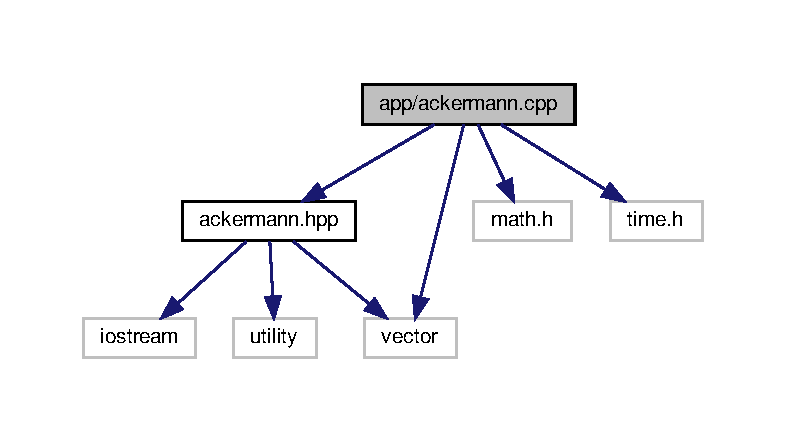
\includegraphics[width=350pt]{ackermann_8cpp__incl}
\end{center}
\end{figure}
\subsection*{Macros}
\begin{DoxyCompactItemize}
\item 
\mbox{\Hypertarget{ackermann_8cpp_a598a3330b3c21701223ee0ca14316eca}\label{ackermann_8cpp_a598a3330b3c21701223ee0ca14316eca}} 
\#define {\bfseries PI}~3.\+141592654
\end{DoxyCompactItemize}


\subsection{Detailed Description}
Phase1-\/ Driver\+: Vivek Sood Navigator\+: Charu Sharma. 

\begin{DoxyAuthor}{Authors}
Vivek Sood, Charu Sharma Phase2-\/ Driver\+: Charu Sharma Navigator\+: Vivek Sood 
\end{DoxyAuthor}

\hypertarget{pid_8cpp}{}\section{app/pid.cpp File Reference}
\label{pid_8cpp}\index{app/pid.\+cpp@{app/pid.\+cpp}}


Driver\+: Vivek Sood Navigator\+: Charu Sharma.  


{\ttfamily \#include $<$pid.\+hpp$>$}\newline
Include dependency graph for pid.\+cpp\+:
\nopagebreak
\begin{figure}[H]
\begin{center}
\leavevmode
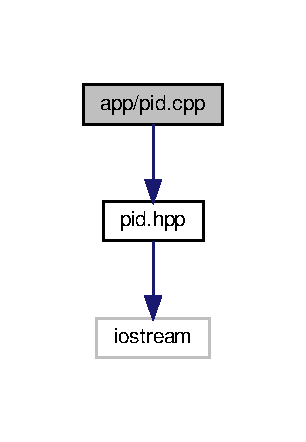
\includegraphics[width=147pt]{pid_8cpp__incl}
\end{center}
\end{figure}


\subsection{Detailed Description}
Driver\+: Vivek Sood Navigator\+: Charu Sharma. 

\begin{DoxyAuthor}{Authors}
Vivek Sood, Charu Sharma 
\end{DoxyAuthor}
\begin{DoxyDate}{Date}
2021-\/10-\/16 
\end{DoxyDate}

\hypertarget{twoWDRobot_8cpp}{}\section{app/two\+W\+D\+Robot.cpp File Reference}
\label{twoWDRobot_8cpp}\index{app/two\+W\+D\+Robot.\+cpp@{app/two\+W\+D\+Robot.\+cpp}}


Driver\+: Vivek Sood Navigator\+: Charu Sharma.  


{\ttfamily \#include \char`\"{}two\+W\+D\+Robot.\+hpp\char`\"{}}\newline
{\ttfamily \#include \char`\"{}pid.\+hpp\char`\"{}}\newline
{\ttfamily \#include \char`\"{}ackermann.\+hpp\char`\"{}}\newline
Include dependency graph for two\+W\+D\+Robot.\+cpp\+:
\nopagebreak
\begin{figure}[H]
\begin{center}
\leavevmode
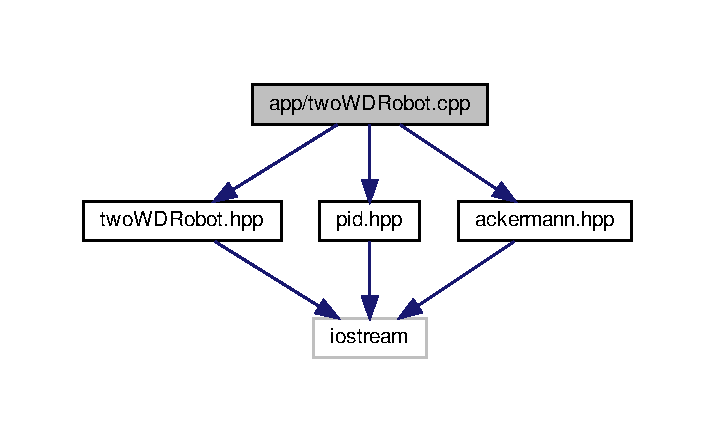
\includegraphics[width=343pt]{twoWDRobot_8cpp__incl}
\end{center}
\end{figure}


\subsection{Detailed Description}
Driver\+: Vivek Sood Navigator\+: Charu Sharma. 

\begin{DoxyAuthor}{Authors}
Vivek Sood, Charu Sharma 
\end{DoxyAuthor}
\begin{DoxyDate}{Date}
2021-\/10-\/16 
\end{DoxyDate}

\hypertarget{ackermann_8hpp}{}\section{include/ackermann.hpp File Reference}
\label{ackermann_8hpp}\index{include/ackermann.\+hpp@{include/ackermann.\+hpp}}


Copyright (c) 2021 Charu Sharma and Vivek Sood.  


{\ttfamily \#include $<$iostream$>$}\newline
{\ttfamily \#include $<$vector$>$}\newline
{\ttfamily \#include $<$utility$>$}\newline
Include dependency graph for ackermann.\+hpp\+:\nopagebreak
\begin{figure}[H]
\begin{center}
\leavevmode
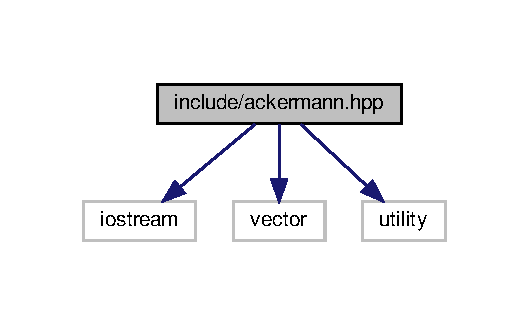
\includegraphics[width=254pt]{ackermann_8hpp__incl}
\end{center}
\end{figure}
This graph shows which files directly or indirectly include this file\+:\nopagebreak
\begin{figure}[H]
\begin{center}
\leavevmode
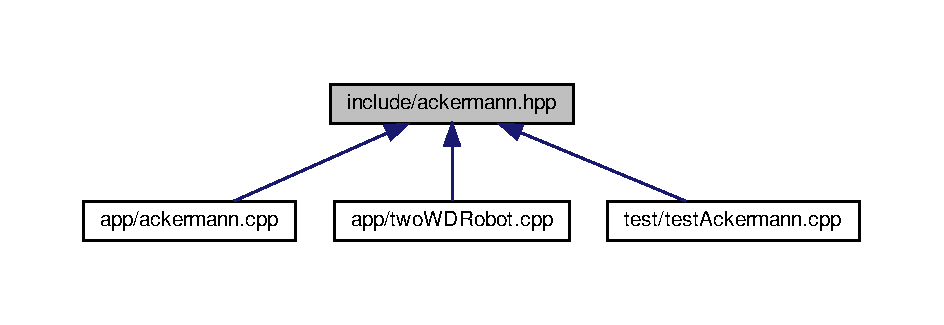
\includegraphics[width=350pt]{ackermann_8hpp__dep__incl}
\end{center}
\end{figure}
\subsection*{Classes}
\begin{DoxyCompactItemize}
\item 
class \hyperlink{classAckermann}{Ackermann}
\begin{DoxyCompactList}\small\item\em Implementation of an \hyperlink{classAckermann}{Ackermann} Controller. \end{DoxyCompactList}\end{DoxyCompactItemize}


\subsection{Detailed Description}
Copyright (c) 2021 Charu Sharma and Vivek Sood. 

\begin{DoxyAuthor}{Authors}
Vivek Sood, Charu Sharma Phase1-\/ Driver\+: Vivek Sood Navigator\+: Charu Sharma Phase2-\/ Driver\+: Charu Sharma Navigator\+: Vivek Sood 
\end{DoxyAuthor}

\hypertarget{pid_8hpp}{}\section{include/pid.hpp File Reference}
\label{pid_8hpp}\index{include/pid.\+hpp@{include/pid.\+hpp}}


Phase1-\/ Driver\+: Vivek Sood Navigator\+: Charu Sharma.  


{\ttfamily \#include $<$iostream$>$}\newline
Include dependency graph for pid.\+hpp\+:\nopagebreak
\begin{figure}[H]
\begin{center}
\leavevmode
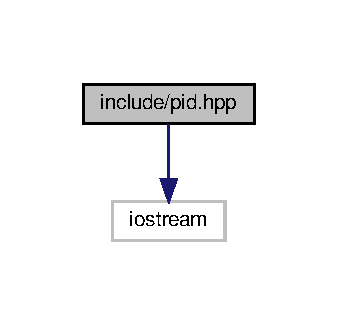
\includegraphics[width=162pt]{pid_8hpp__incl}
\end{center}
\end{figure}
This graph shows which files directly or indirectly include this file\+:\nopagebreak
\begin{figure}[H]
\begin{center}
\leavevmode
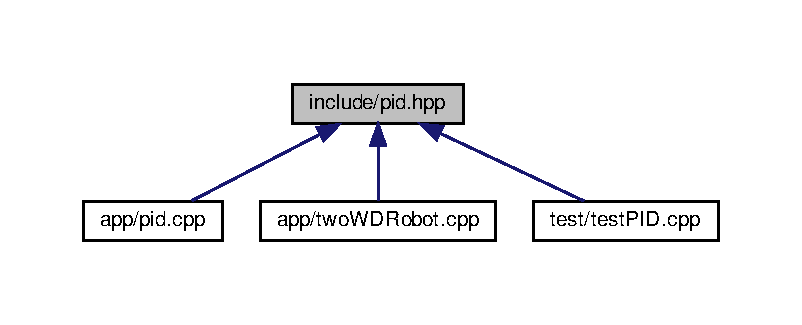
\includegraphics[width=350pt]{pid_8hpp__dep__incl}
\end{center}
\end{figure}
\subsection*{Classes}
\begin{DoxyCompactItemize}
\item 
class \hyperlink{classPID}{P\+ID}
\begin{DoxyCompactList}\small\item\em Implementation of a \hyperlink{classPID}{P\+ID} controller. \end{DoxyCompactList}\end{DoxyCompactItemize}


\subsection{Detailed Description}
Phase1-\/ Driver\+: Vivek Sood Navigator\+: Charu Sharma. 

\begin{DoxyAuthor}{Authors}
Vivek Sood, Charu Sharma Phase2-\/ Driver\+: Charu Sharma Navigator\+: Vivek Sood 
\end{DoxyAuthor}

\hypertarget{twoWDRobot_8hpp}{}\section{include/two\+W\+D\+Robot.hpp File Reference}
\label{twoWDRobot_8hpp}\index{include/two\+W\+D\+Robot.\+hpp@{include/two\+W\+D\+Robot.\+hpp}}


Driver\+: Vivek Sood Navigator\+: Charu Sharma.  


{\ttfamily \#include $<$iostream$>$}\newline
Include dependency graph for two\+W\+D\+Robot.\+hpp\+:\nopagebreak
\begin{figure}[H]
\begin{center}
\leavevmode
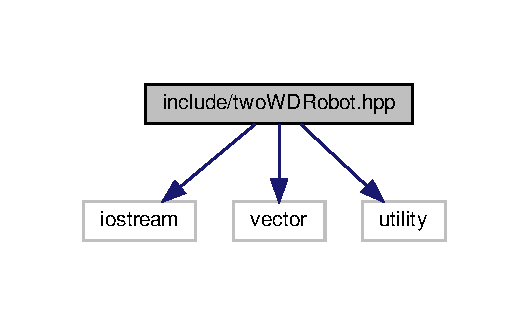
\includegraphics[width=208pt]{twoWDRobot_8hpp__incl}
\end{center}
\end{figure}
This graph shows which files directly or indirectly include this file\+:\nopagebreak
\begin{figure}[H]
\begin{center}
\leavevmode
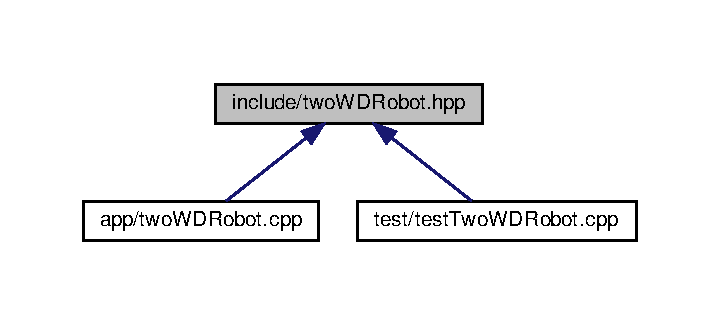
\includegraphics[width=346pt]{twoWDRobot_8hpp__dep__incl}
\end{center}
\end{figure}
\subsection*{Classes}
\begin{DoxyCompactItemize}
\item 
class \hyperlink{classTwoWDRobot}{Two\+W\+D\+Robot}
\begin{DoxyCompactList}\small\item\em Implementation of an \hyperlink{classTwoWDRobot}{Two\+W\+D\+Robot} Class. \end{DoxyCompactList}\end{DoxyCompactItemize}


\subsection{Detailed Description}
Driver\+: Vivek Sood Navigator\+: Charu Sharma. 

\begin{DoxyAuthor}{Authors}
Vivek Sood, Charu Sharma 
\end{DoxyAuthor}
\begin{DoxyDate}{Date}
2021-\/10-\/16 
\end{DoxyDate}

\hypertarget{visualization_8hpp}{}\section{include/visualization.hpp File Reference}
\label{visualization_8hpp}\index{include/visualization.\+hpp@{include/visualization.\+hpp}}


Driver\+: Vivek Sood Navigator\+: Charu Sharma.  


{\ttfamily \#include $<$iostream$>$}\newline
{\ttfamily \#include $<$vector$>$}\newline
Include dependency graph for visualization.\+hpp\+:\nopagebreak
\begin{figure}[H]
\begin{center}
\leavevmode
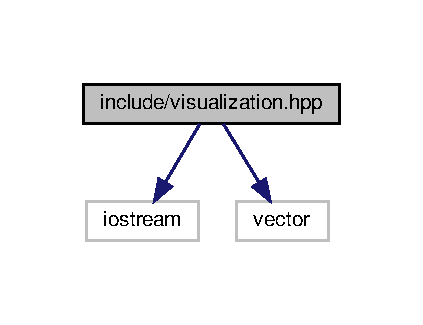
\includegraphics[width=203pt]{visualization_8hpp__incl}
\end{center}
\end{figure}
This graph shows which files directly or indirectly include this file\+:\nopagebreak
\begin{figure}[H]
\begin{center}
\leavevmode
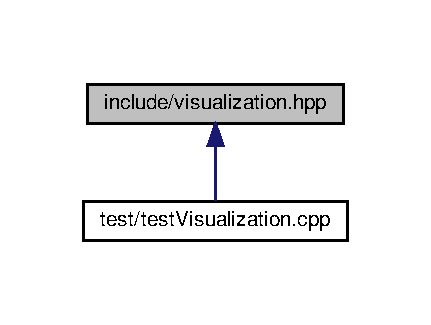
\includegraphics[width=207pt]{visualization_8hpp__dep__incl}
\end{center}
\end{figure}
\subsection*{Classes}
\begin{DoxyCompactItemize}
\item 
class \hyperlink{classVisualization}{Visualization}
\begin{DoxyCompactList}\small\item\em Implementation of an \hyperlink{classVisualization}{Visualization} Class. \end{DoxyCompactList}\end{DoxyCompactItemize}


\subsection{Detailed Description}
Driver\+: Vivek Sood Navigator\+: Charu Sharma. 

\begin{DoxyAuthor}{Authors}
Vivek Sood, Charu Sharma 
\end{DoxyAuthor}
\begin{DoxyDate}{Date}
2021-\/10-\/17 
\end{DoxyDate}

\hypertarget{testAckermann_8cpp}{}\section{test/test\+Ackermann.cpp File Reference}
\label{testAckermann_8cpp}\index{test/test\+Ackermann.\+cpp@{test/test\+Ackermann.\+cpp}}
{\ttfamily \#include $<$gtest/gtest.\+h$>$}\newline
{\ttfamily \#include \char`\"{}ackermann.\+hpp\char`\"{}}\newline
Include dependency graph for test\+Ackermann.\+cpp\+:
\nopagebreak
\begin{figure}[H]
\begin{center}
\leavevmode
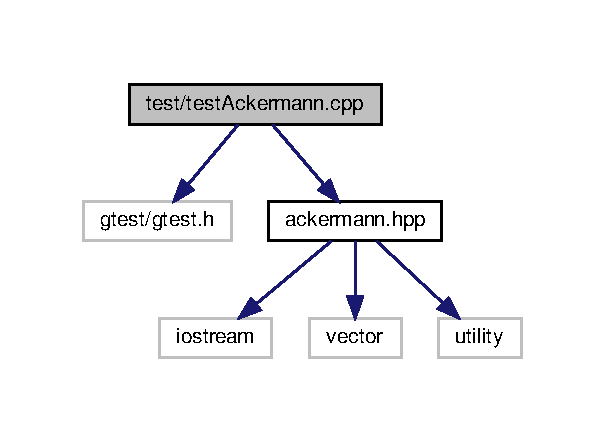
\includegraphics[width=252pt]{testAckermann_8cpp__incl}
\end{center}
\end{figure}
\subsection*{Functions}
\begin{DoxyCompactItemize}
\item 
\mbox{\Hypertarget{testAckermann_8cpp_ab93bec5a0d8f561fc795d75e165bbdbe}\label{testAckermann_8cpp_ab93bec5a0d8f561fc795d75e165bbdbe}} 
{\bfseries T\+E\+ST} (Ackermann\+Tests, test\+Set\+Attributes)
\item 
\mbox{\Hypertarget{testAckermann_8cpp_aa350b17ab7e59e4c6cc82b101baee0fd}\label{testAckermann_8cpp_aa350b17ab7e59e4c6cc82b101baee0fd}} 
{\bfseries T\+E\+ST} (Ackermann\+Tests, test\+Compute\+Model\+Outputs)
\end{DoxyCompactItemize}
\subsection*{Variables}
\begin{DoxyCompactItemize}
\item 
\mbox{\Hypertarget{testAckermann_8cpp_a67296585483cc8e5db36cd42d66266fe}\label{testAckermann_8cpp_a67296585483cc8e5db36cd42d66266fe}} 
\hyperlink{classAckermann}{Ackermann} {\bfseries ackermann}
\end{DoxyCompactItemize}


\subsection{Detailed Description}
\begin{DoxyAuthor}{Authors}
Vivek Sood and Charu Sharma 
\end{DoxyAuthor}
\begin{DoxyDate}{Date}
2021-\/10-\/05 
\end{DoxyDate}
\begin{DoxyCopyright}{Copyright}
Copyright (c) 2021
\end{DoxyCopyright}
E\+N\+P\+M808X Midterm -\/ Phase 0 Proposal 
\hypertarget{testPID_8cpp}{}\section{test/test\+P\+ID.cpp File Reference}
\label{testPID_8cpp}\index{test/test\+P\+I\+D.\+cpp@{test/test\+P\+I\+D.\+cpp}}


main file for testing  


{\ttfamily \#include $<$gtest/gtest.\+h$>$}\newline
{\ttfamily \#include \char`\"{}pid.\+hpp\char`\"{}}\newline
Include dependency graph for test\+P\+I\+D.\+cpp\+:\nopagebreak
\begin{figure}[H]
\begin{center}
\leavevmode
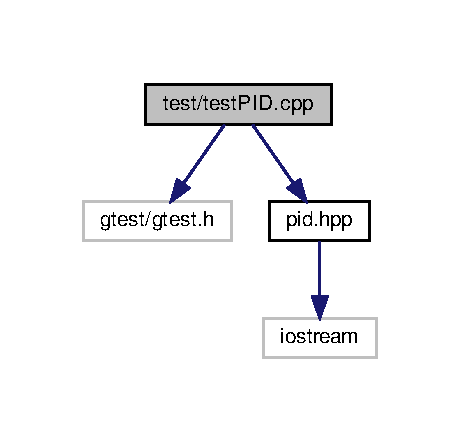
\includegraphics[width=221pt]{testPID_8cpp__incl}
\end{center}
\end{figure}
\subsection*{Functions}
\begin{DoxyCompactItemize}
\item 
\mbox{\Hypertarget{testPID_8cpp_af16905d97ee29751033c9b0daa2be7a7}\label{testPID_8cpp_af16905d97ee29751033c9b0daa2be7a7}} 
{\bfseries T\+E\+ST} (\hyperlink{classPID}{P\+ID}, test\+Set\+Attributes)
\item 
\mbox{\Hypertarget{testPID_8cpp_a3f6f58b239babf08620ba12d443cddb1}\label{testPID_8cpp_a3f6f58b239babf08620ba12d443cddb1}} 
{\bfseries T\+E\+ST} (\hyperlink{classPID}{P\+ID}, test\+Compute\+P\+ID)
\end{DoxyCompactItemize}
\subsection*{Variables}
\begin{DoxyCompactItemize}
\item 
\mbox{\Hypertarget{testPID_8cpp_a748a9dfe6ca5dbeb9bfb514f5d753ffe}\label{testPID_8cpp_a748a9dfe6ca5dbeb9bfb514f5d753ffe}} 
\hyperlink{classPID}{P\+ID} {\bfseries pid}
\end{DoxyCompactItemize}


\subsection{Detailed Description}
main file for testing 

\begin{DoxyAuthor}{Authors}
Vivek Sood and Charu Sharma 
\end{DoxyAuthor}
\begin{DoxyDate}{Date}
2021-\/10-\/16 
\end{DoxyDate}
\begin{DoxyCopyright}{Copyright}
Copyright (c) 2021
\end{DoxyCopyright}
E\+N\+P\+M808X Midterm -\/ Phase 1 
\hypertarget{testTwoWDRobot_8cpp}{}\section{test/test\+Two\+W\+D\+Robot.cpp File Reference}
\label{testTwoWDRobot_8cpp}\index{test/test\+Two\+W\+D\+Robot.\+cpp@{test/test\+Two\+W\+D\+Robot.\+cpp}}
{\ttfamily \#include $<$gtest/gtest.\+h$>$}\newline
{\ttfamily \#include \char`\"{}two\+W\+D\+Robot.\+hpp\char`\"{}}\newline
Include dependency graph for test\+Two\+W\+D\+Robot.\+cpp\+:\nopagebreak
\begin{figure}[H]
\begin{center}
\leavevmode
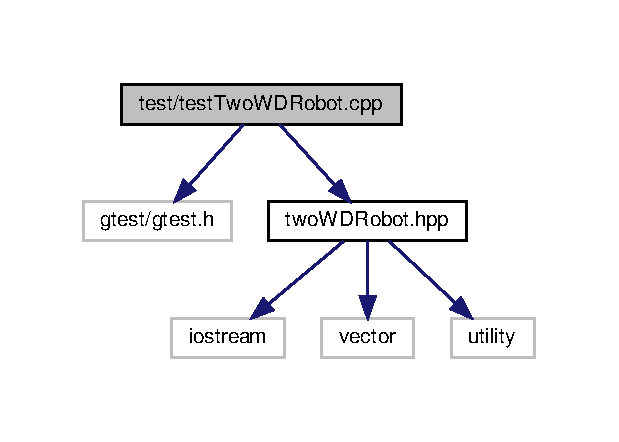
\includegraphics[width=264pt]{testTwoWDRobot_8cpp__incl}
\end{center}
\end{figure}
\subsection*{Functions}
\begin{DoxyCompactItemize}
\item 
\mbox{\Hypertarget{testTwoWDRobot_8cpp_a1ffa7d6585ab039c4c339f90718002f8}\label{testTwoWDRobot_8cpp_a1ffa7d6585ab039c4c339f90718002f8}} 
{\bfseries T\+E\+ST} (Two\+W\+D\+Robot\+Tests, test\+Set\+Attributes)
\item 
\mbox{\Hypertarget{testTwoWDRobot_8cpp_aa17f477f4fb42e0b0704dfeaadb30d70}\label{testTwoWDRobot_8cpp_aa17f477f4fb42e0b0704dfeaadb30d70}} 
{\bfseries T\+E\+ST} (Two\+W\+D\+Robot\+Tests, testcompute\+Heading)
\item 
\mbox{\Hypertarget{testTwoWDRobot_8cpp_a061bda583e7dbc81d83e08370c54580b}\label{testTwoWDRobot_8cpp_a061bda583e7dbc81d83e08370c54580b}} 
{\bfseries T\+E\+ST} (Two\+W\+D\+Robot\+Tests, testcompute\+Velocity)
\end{DoxyCompactItemize}
\subsection*{Variables}
\begin{DoxyCompactItemize}
\item 
\mbox{\Hypertarget{testTwoWDRobot_8cpp_aed98d72824089c5da928d7a7136f00a1}\label{testTwoWDRobot_8cpp_aed98d72824089c5da928d7a7136f00a1}} 
\hyperlink{classTwoWDRobot}{Two\+W\+D\+Robot} {\bfseries two\+W\+D\+Robot}
\end{DoxyCompactItemize}


\subsection{Detailed Description}
\begin{DoxyAuthor}{Authors}
Vivek Sood and Charu Sharma 
\end{DoxyAuthor}
\begin{DoxyDate}{Date}
2021-\/10-\/17 
\end{DoxyDate}
\begin{DoxyCopyright}{Copyright}
Copyright (c) 2021
\end{DoxyCopyright}
E\+N\+P\+M808X Midterm -\/ Phase 0 Proposal 
\hypertarget{testVisualization_8cpp}{}\section{test/test\+Visualization.cpp File Reference}
\label{testVisualization_8cpp}\index{test/test\+Visualization.\+cpp@{test/test\+Visualization.\+cpp}}
{\ttfamily \#include $<$gtest/gtest.\+h$>$}\newline
{\ttfamily \#include $<$vector$>$}\newline
{\ttfamily \#include \char`\"{}visualization.\+hpp\char`\"{}}\newline
Include dependency graph for test\+Visualization.\+cpp\+:
\nopagebreak
\begin{figure}[H]
\begin{center}
\leavevmode
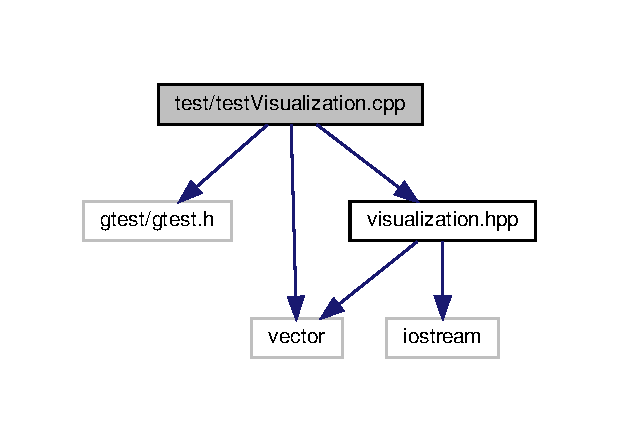
\includegraphics[width=297pt]{testVisualization_8cpp__incl}
\end{center}
\end{figure}
\subsection*{Functions}
\begin{DoxyCompactItemize}
\item 
\mbox{\Hypertarget{testVisualization_8cpp_aaa85c9edf8d68ee2010207c9085401cc}\label{testVisualization_8cpp_aaa85c9edf8d68ee2010207c9085401cc}} 
{\bfseries T\+E\+ST} (visualization\+Tests, test\+Set\+Attributes)
\item 
\mbox{\Hypertarget{testVisualization_8cpp_a9ee123d29b80a6f55133f6f4d2480d31}\label{testVisualization_8cpp_a9ee123d29b80a6f55133f6f4d2480d31}} 
{\bfseries T\+E\+ST} (visualization\+Tests, test\+Plot\+Velocities)
\item 
\mbox{\Hypertarget{testVisualization_8cpp_abe29f73ed967d10a88b7d4ffc366e0ac}\label{testVisualization_8cpp_abe29f73ed967d10a88b7d4ffc366e0ac}} 
{\bfseries T\+E\+ST} (visualization\+Tests, testcompute\+Heading)
\end{DoxyCompactItemize}
\subsection*{Variables}
\begin{DoxyCompactItemize}
\item 
\mbox{\Hypertarget{testVisualization_8cpp_a10cd776bed271ba72660c928eb8147ff}\label{testVisualization_8cpp_a10cd776bed271ba72660c928eb8147ff}} 
\hyperlink{classVisualization}{Visualization} {\bfseries visualization}
\end{DoxyCompactItemize}


\subsection{Detailed Description}
\begin{DoxyAuthor}{Authors}
Vivek Sood and Charu Sharma 
\end{DoxyAuthor}
\begin{DoxyDate}{Date}
2021-\/10-\/18 
\end{DoxyDate}
\begin{DoxyCopyright}{Copyright}
Copyright (c) 2021
\end{DoxyCopyright}
E\+N\+P\+M808X Midterm -\/ Phase 1 
%--- End generated contents ---

% Index
\backmatter
\newpage
\phantomsection
\clearemptydoublepage
\addcontentsline{toc}{chapter}{Index}
\printindex

\end{document}
